% Define table for personas.
\newcommand{\persona}[4]{%
    \textbf{#1}
    \small\begin{tabular}[t]{|p{.8in} | p{1.5in}|}
        \hline
        \textbf{Preferences} & #2 \\\hline
        \textbf{Pain Points} & #3 \\\hline
        \textbf{Goals} & #4 \\
        \hline
    \end{tabular}
    \vspace{4pt}
}


\chapter{Introduction}
\label{chap:introduction}

\section{Background}
\label{section:background}

In modern surveillance systems, the ability to track individuals across multiple camera views is crucial for security and analytics applications.
Traditional surveillance methods rely heavily on human operators monitoring multiple screens simultaneously, which is both labor-intensive and prone to error.
As the number of cameras in surveillance networks increases, the challenge of effectively monitoring and tracking individuals becomes exponentially more difficult.
The limitations of manual surveillance include operator fatigue, inconsistent identification, and the inability to quickly locate specific individuals across diverse environments. \cite{surveillanceetal:2023}

In commercial and industrial settings such as retail stores, office buildings, cafes, industrial facilities, and lobbies,
the need for intelligent surveillance systems that can automatically identify and track individuals of interest is significant.
Current systems often struggle with maintaining consistent identification when subjects move between camera views,
especially in crowded scenes or when individuals change appearance or direction. This creates substantial gaps in surveillance coverage
and reduces the effectiveness of security measures in these environments.

The advancement of artificial intelligence, particularly in computer vision and machine learning,
has opened new possibilities for addressing these challenges. Technologies such as real-time object detection,
person re-identification, and large language models can be integrated to create more intelligent and responsive surveillance systems.
However, these technologies have not yet been fully leveraged in a cohesive, user-friendly system that meets the needs of security professionals
monitoring diverse indoor environments like those represented in the MMPTrack dataset.

\section{Problem Statement}
\label{section:problem-statement}

The Intelligent Multi-Camera Person Tracking and Analytics System addresses several critical technical challenges in modern surveillance systems. First, detecting and identifying the same individual across multiple cameras with varying angles, lighting conditions, and occlusions remains highly complex. Current systems struggle with consistent re-identification when subjects appear in different camera views, particularly when individuals share similar physical attributes or clothing. Second, while Large Language Models show promise for natural language-based person filtering, their application in real-world surveillance scenarios lacks robust validation and standardized implementation approaches. Third, perspective transformation—mapping individuals from different camera views onto a unified coordinate system—presents significant technical hurdles due to varying camera positions, lens distortions, and environmental factors. Fourth, the integration of these technologies into a cohesive, real-time system that security personnel can effectively utilize requires overcoming substantial engineering challenges in data synchronization, processing latency, and user interface design. These challenges are particularly evident in diverse indoor environments such as retail spaces, offices, industrial facilities, cafes, and lobbies, where existing solutions fail to provide the seamless, intuitive tracking capabilities required by security professionals.

\section{Solution Overview}
\label{section:solution-overview}

The Intelligent Multi-Camera Person Tracking and Analytics System proposes a solution by being an AI-powered surveillance platform
that is designed for security professionals with four prominent features and additional capabilities to solve the problem,

\subsection{Prominent Features}
\label{subsection:main-features}

\begin{enumerate}[leftmargin=80pt]
    \item \textbf{LLM-Powered Person Selection:} A natural language interface that allows users to identify individuals
    based on descriptive prompts (e.g., "Find the person wearing a red shirt and carrying a backpack"), enhancing the speed
    and accuracy of subject identification in diverse indoor environments.
    \item \textbf{Real-Time Person Detection and Re-Identification:} An advanced object detection system that maintains
    consistent identification of individuals across multiple camera views in retail, office, industrial, cafe, and lobby settings,
    even when they temporarily leave one camera's field of view and appear in another.
    \item \textbf{Path Tracking and Visualization:} A dynamic mapping system that plots the movement of tracked individuals
    across multiple camera views within indoor environments, providing clear visualization of their paths with timestamps and key locations.
    \item \textbf{Zoom and Focus Capabilities:} A system that allows users to click on a person or object in the video feed
    to zoom in and focus on them in real time, enhancing visibility and detail for critical observations in various indoor settings.
\end{enumerate}

\subsection{Technical Implementation}
\label{subsection:technical-implementation}

\begin{enumerate}[leftmargin=80pt]
    \item \textbf{Object Detection and Tracking} \\%
        The system employs state-of-the-art detection and tracking technologies:
        \begin{enumerate}
            \item YOLOv11 for real-time object detection—providing optimal speed and efficiency for surveillance applications in indoor environments.
            \item ByteTrack for robust tracking—handling occlusions and maintaining identity consistency in crowded indoor scenes.
        \end{enumerate}
    \item \textbf{Re-Identification and LLM Integration} \\%
        Advanced technologies ensure accurate subject identification across camera views:
        \begin{enumerate}
            \item FastReID for person re-identification—maintaining consistent identity across different camera perspectives in varied indoor settings.
            \item OpenCLIP for natural language processing—enabling description-based person selection through intuitive prompts tailored to retail, office, industrial, cafe, and lobby environments.
        \end{enumerate}
\end{enumerate}

\subsection{Optional Features}
\label{subsection:optional-features}

\begin{enumerate}[leftmargin=80pt]
    \item \textbf{Multi-Object Tracking:} Capability to simultaneously track multiple individuals or objects across the surveillance network in diverse indoor environments.
    \item \textbf{Behavior Prediction:} AI-powered analysis to predict movement patterns and provide early warnings for unusual behavior in specific contexts like retail theft prevention or industrial safety monitoring.
    \item \textbf{Dynamic Analytics:} Real-time metrics including walking speed, time spent in specific areas, and movement pattern heatmaps customized for retail, office, industrial, cafe, and lobby settings.
    \item \textbf{Automatic Map Generation:} System that creates maps based on observed movement patterns in indoor environments, eliminating the need for manual mapping.
\end{enumerate}

\section{Target User}
\label{section:target-user}

The overarching goal for the Intelligent Multi-Camera Person Tracking and Analytics System is to provide security professionals
with a powerful, intuitive tool for monitoring and analyzing surveillance footage across multiple camera views in diverse indoor environments.
By leveraging advanced AI technologies, the system aims to enhance security operations, reduce response times,
and provide actionable insights that improve overall safety and security in retail, office, industrial, cafe, and lobby settings.

The primary users of the system are security professionals responsible for surveillance monitoring and response in these environments.
Below are examples of the diverse users who can benefit from our system.

\begin{table}[p]
    \centering
    \noindent\begin{tabular}{| p{2.65in} | p{2.65in} |}
        \hline & \\[-10pt]
        \persona{Retail Security Manager}
        {Real-time tracking capabilities, intuitive interfaces, theft prevention tools specific to retail environments.}
        {Overwhelmed by multiple CCTV feeds, difficulty identifying suspicious behavior in crowded stores.}
        {To quickly locate and track persons of interest across retail spaces and coordinate rapid response to potential theft or security incidents.} &
        \persona{Office Building Security Officer}
        {Access control integration, visitor tracking, minimal disruption to professional environments.}
        {Managing security across multiple floors and office spaces, identifying unauthorized visitors.}
        {To efficiently monitor building access points and common areas while maintaining a professional, unobtrusive security presence.} \\[10pt]
        \hline & \\[-10pt]
        \persona{Industrial Safety Supervisor}
        {Safety protocol monitoring, hazard zone tracking, integration with industrial safety systems.}
        {Ensuring worker compliance with safety protocols, monitoring restricted areas in industrial settings.}
        {To identify safety violations, track personnel in hazardous areas, and improve overall workplace safety through data-driven insights.} &
        \persona{Commercial Property Manager}
        {System reliability, comprehensive dashboard views, multi-environment monitoring capabilities.}
        {Coordinating security across diverse spaces (lobbies, cafes, offices), balancing security with customer experience.}
        {To improve operational efficiency, reduce security incidents, and maintain comprehensive situational awareness across all monitored areas.} \\[10pt]
        \hline
    \end{tabular}
    \caption{Personas from User Analysis for Intelligent Multi-Camera Person Tracking System}
\end{table}

\newpage

\section{Benefit}
\label{section:benefit}

The benefits of the Intelligent Multi-Camera Person Tracking and Analytics System include enhanced security operations
with faster subject identification and tracking in diverse indoor environments, reduced response times through real-time alerts and path visualization,
and more efficient resource allocation for security personnel.

The system also offers improved investigative capabilities with comprehensive movement tracking and analytics tailored to specific environments,
reduced operator fatigue through AI-assisted monitoring, and scalable surveillance coverage that can adapt to
retail, office, industrial, cafe, and lobby settings of varying sizes and complexities.

\section{Timeline}
\label{section:timeline}

\begin{figure}[h!]
    \centering
    % 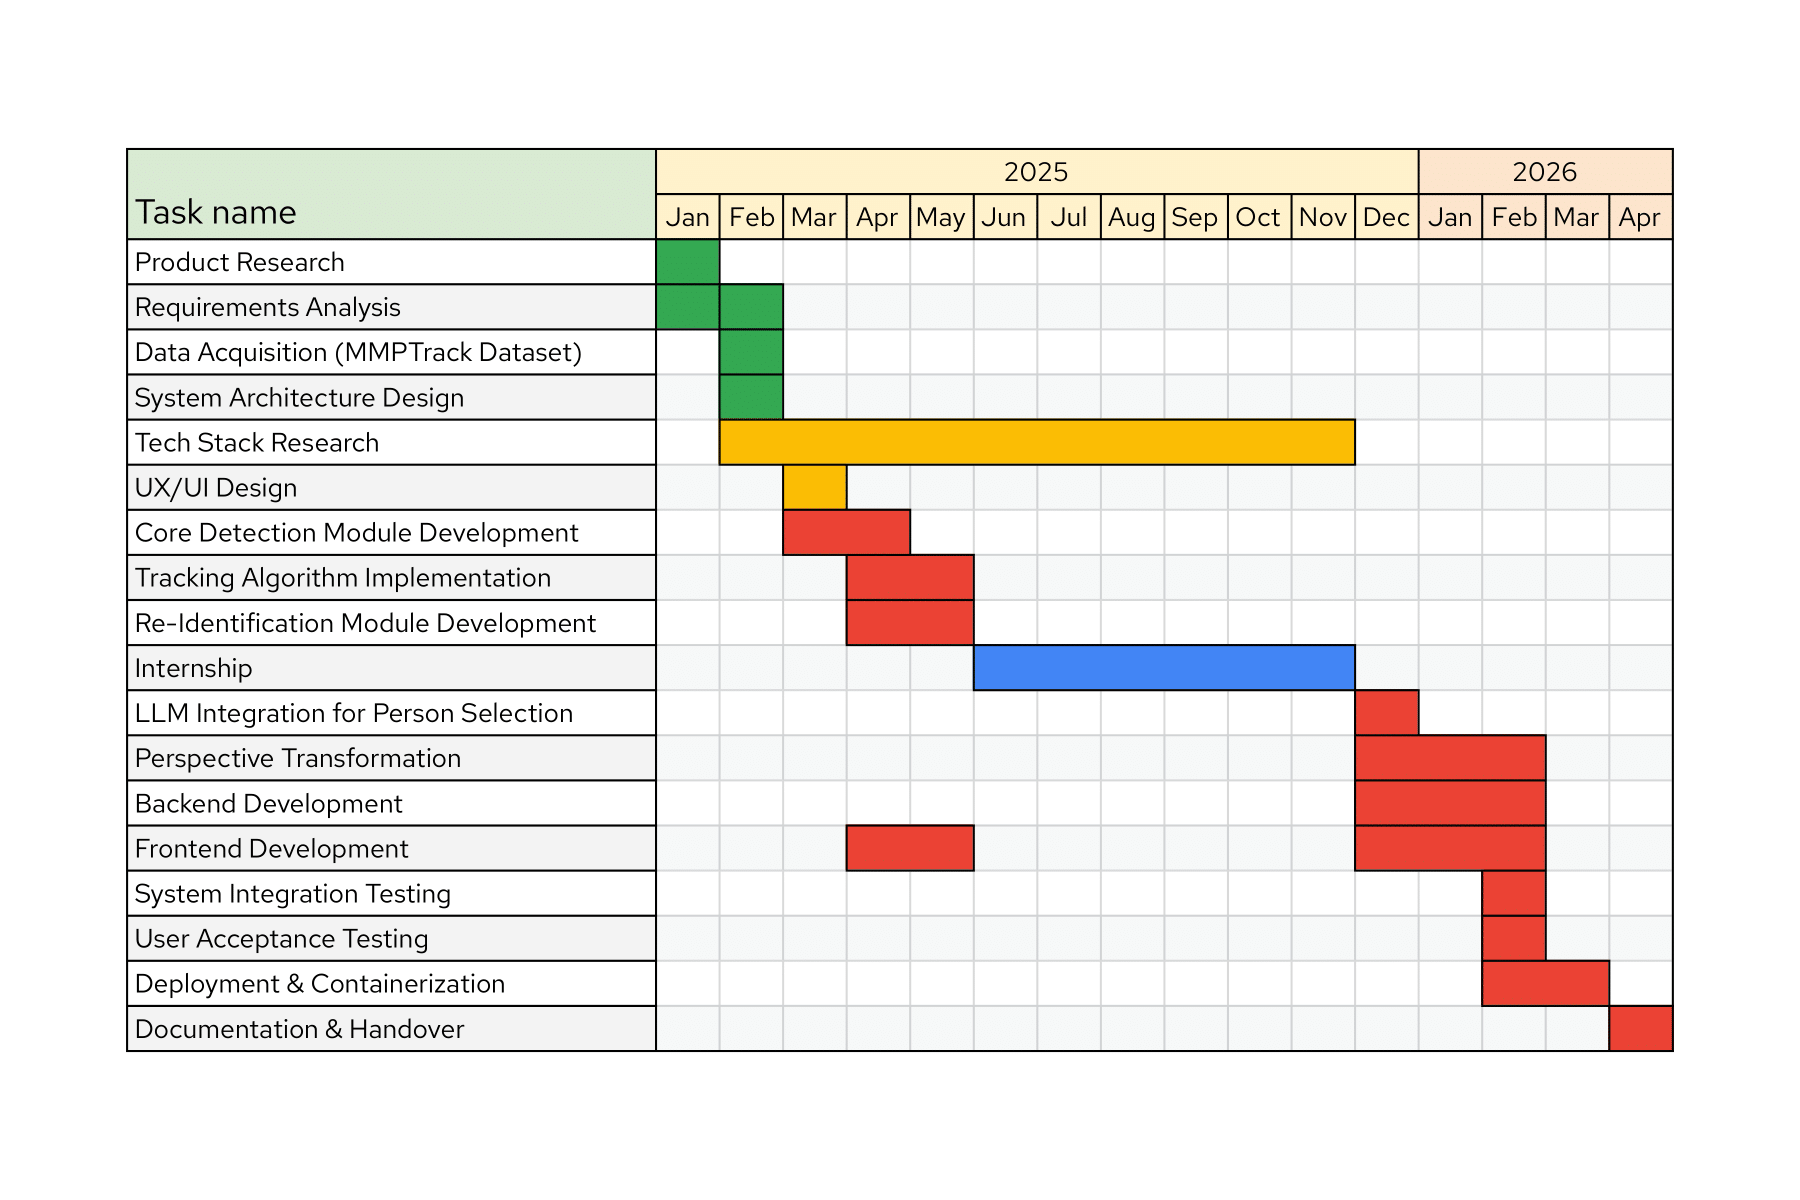
\includegraphics[width=\textwidth,height=0.5\textheight,keepaspectratio]{tracking/timeline.png}
    \caption{Timeline for Intelligent Multi-Camera Person Tracking System Project}
    \label{fig:timeline}
\end{figure}

As shown in figure \ref{fig:timeline}, it represents the timeline of the project.
The project began with system architecture design in January 2025, followed by the development of core detection
and tracking modules in February 2025. The re-identification and LLM integration components are scheduled for
completion by mid-March 2025.

System integration testing will commence in late March 2025, with user acceptance testing planned for early April 2025.
The final deployment and handover are scheduled for completion by the end of April 2025, with ongoing support
and maintenance to follow.

\section{Terminology}
\label{section:terminology}

\begin{itemize}[leftmargin=40pt]
    \item \textbf{\textit{Object Detection}}---a computer vision technique that identifies and locates objects within digital images or video frames.
    \item \textbf{\textit{Re-Identification (Re-ID)}}---the process of matching individuals across different camera views based on their appearance and other characteristics.
    \item \textbf{\textit{Large Language Model (LLM)}}---an advanced AI system trained on vast amounts of text data that can understand and generate human-like text, enabling natural language interactions.
    \item \textbf{\textit{Perspective Transformation}}---a technique that converts camera views to a standardized perspective, typically a top-down view, to enable accurate mapping and tracking.
    \item \textbf{\textit{Multi-Object Tracking (MOT)}}---a computer vision task that involves detecting multiple objects in video frames and tracking them over time while maintaining their identities.
    \item \textbf{\textit{MMPTrack Dataset}}---a multi-camera tracking dataset featuring synchronized video from diverse indoor environments including retail spaces, offices, industrial facilities, cafes, and lobbies.
\end{itemize}